\documentclass[11pt,a4paper]{article}
\usepackage{harmonikabau_preamble}

% == Document metadata ====================
\newcommand{\hbdoknr}{0002}
\newcommand{\hbtitel}{Flow Analysis of a 50\,Hz Bass Reed}
\newcommand{\hbuntertitel}{v8 -- v7 base + slot entry loss (K3b) + dynamic gap change (K6)}
\newcommand{\hbheadtext}{Doc.\,0002 --- Flow Analysis: 50\,Hz Bass Reed -- v8}
\newcommand{\hbfoottext}{Stationary \& non-stationary analysis}

\AtBeginDocument{%
  \fancyhead[L]{\small\hbheadtext}%
  \fancyhead[R]{\small\thepage}%
  \fancyfoot[C]{\small\color{hb@darkgray}\hbfoottext}%
}

\begin{document}
\hbmaketitle

{\small\itshape Corrections relative to v6: (1) gap area $W \cdot h/3$ instead of $W \cdot h/2$ (cantilever profile), (2) laminar friction $f=64/\text{Re}$ instead of $f=0.03$, (3) threshold pressure $8EIh/(WL^4)$, (4) Helmholtz with slot as neck, (5) Reynolds numbers stated throughout. New in v8: (K3b) slot entry loss $\zeta_\text{entry}=0.5$ added, (K6) static gap narrowing under bellows pressure with critical pressure $\Delta p_\text{crit}$.}

\vspace{4mm}

% ============================================================
\section{Construction}
% ============================================================

\begin{keybox}
In the bass section of an accordion, dozens of reeds sit in individual chambers, all connected to the same bellows. The bellows generates the pressure; the keys control the valves via mechanical levers. The valve is \textbf{not} opened by bellows pressure -- pressure acts on all closed valves simultaneously. Only pressing a key opens the valve mechanically.
\end{keybox}

% ============================================================
\section{Chamber, Reed Plate, and Offset}
% ============================================================

The chamber is a wooden block measuring $94 \times 48 \times 40$\,mm. The entire top surface is sealed by an aluminium reed plate. This plate is \textbf{wedge-shaped}: 13\,mm thick at the free reed tip (above the valve), only 2\,mm at the clamping end. The slot in the plate is therefore 13\,mm deep at the free end -- air must traverse a short channel before reaching the reed.

The steel reed ($70 \times 8 \times 0.354$\,mm) is fastened to the plate with \textbf{two screws} (smaller reed plates are riveted). The free end is \textbf{offset by 1.5\,mm} -- at rest it stands 1.5\,mm above the plate surface. This creates a triangular gap: 0\,mm at the clamp, 1.5\,mm at the free tip.

The effective gap area accounts for the cantilever bending profile $y(x) \sim y_\text{tip} \cdot (x/L)^2$. The gap is largest at the tip and decreases quadratically:
\begin{equation}
S_\text{gap} = \frac{W \cdot h_\text{max}}{3} = \frac{8 \times 1.5}{3} = \mathbf{4\,\text{mm}^2}
\end{equation}
(v6 used factor $1/2 = 6\,\text{mm}^2$ -- linear profile.) For comparison: the valve opening area is approx.\ 244\,mm$^2$ -- about 61 times larger. The gap remains the bottleneck.

\begin{figure}[H]
\centering
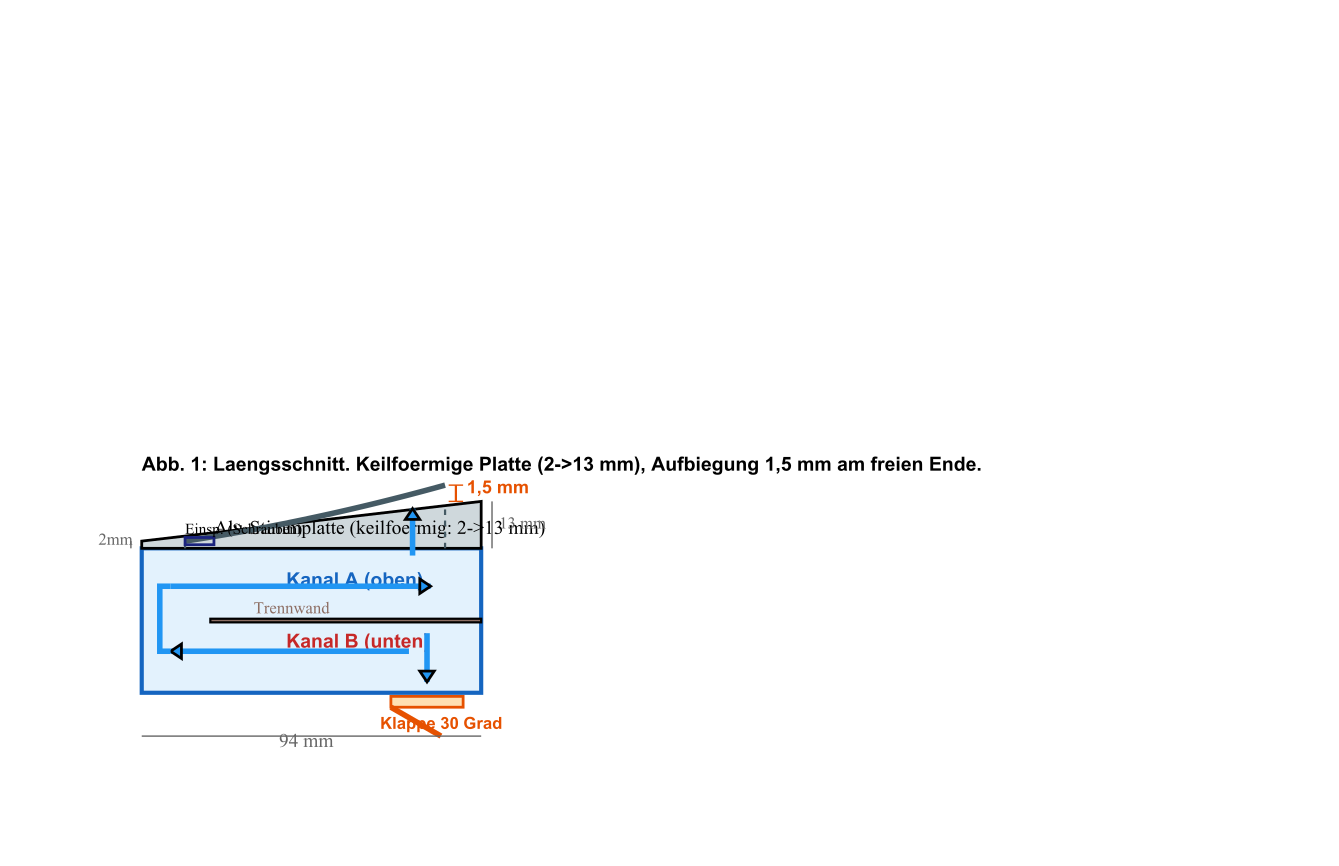
\includegraphics[width=\textwidth]{abb1_laengsschnitt.png}
\caption{Longitudinal cross-section of the reed.
  Wedge-shaped plate (2\,$\rightarrow$\,13\,mm thickness),
  1.5\,mm offset at the free tip.
  The gap (grey) is largest at the tip and decreases quadratically towards the clamp.}
\end{figure}

% ============================================================
\section{The Folded Air Path}
% ============================================================

A dividing wall splits the chamber into two channels. The air path:

\medskip
\begin{center}
Valve (floor, right) $\rightarrow$ Channel B leftward $\rightarrow$\\
180°\,fold $\rightarrow$ Channel A rightward $\rightarrow$ Slot $\rightarrow$ Gap
\end{center}
\medskip

Total path length over 200\,mm.

% ============================================================
\section{Dividing Wall -- Film or Veneer?}
% ============================================================

Two materials are suitable for the dividing wall: \textbf{plastic film} ($\sim$0.3\,mm) or \textbf{wood veneer} ($\sim$0.5\,mm). Wall thickness affects channel width: with a straight wall, film gives 23.85\,mm per channel, veneer 23.75\,mm -- a difference of 0.10\,mm (0.4\,\%). This is negligible from a flow perspective.

\begin{table}[H]
\centering\small
\resizebox{\linewidth}{!}{\begin{tabular}{l l l}
\toprule
& \textbf{Film (0.3\,mm)} & \textbf{Veneer (0.5\,mm)} \\
\midrule
Surface & Smooth $\rightarrow$ less friction ($f \approx 0.02$) & Rough $\rightarrow$ more friction ($f \approx 0.03$) \\
Stability & Flexible $\rightarrow$ can flutter, needs support & Dimensionally stable $\rightarrow$ holds position \\
Acoustics & Can vibrate as a membrane $\rightarrow$ noise & Acoustically inert \\
Installation & Gluing, tensioning & Gluing, clamping, easier \\
\bottomrule
\end{tabular}}
\caption{Film vs.\ veneer as dividing wall material}
\end{table}

Since channel friction constitutes a negligible fraction of total losses, the friction difference between film and veneer is irrelevant for flow. The difference lies solely in stability and acoustics. Veneer is the safer choice; film is only appropriate when space is extremely tight.

% ============================================================
\section{Valve Orientation -- Blow-out or Deflect?}
% ============================================================

\textbf{Blow-out direction:} The valve opens so that the 30° jet points directly into Channel B. The jet has a horizontal component of 87\,\% and a vertical component of 50\,\%. Loss coefficient: $\zeta_\text{valve} = 0.498$ (vena contracta + direction change).

\textbf{Deflect direction:} The valve opens outwards. Air must turn $\sim$150° around the valve edge before entering the chamber. Loss coefficient: $\zeta_\text{valve} = 1.698$ -- \textbf{3.4 times} the blow-out direction.

\begin{table}[H]
\centering\small
\resizebox{\linewidth}{!}{\begin{tabular}{l l l}
\toprule
& \textbf{Blow-out} & \textbf{Deflect} \\
\midrule
Jet & Directed into chamber & First away, then 150°\,turn \\
$\zeta_\text{valve}$ & 0.498 & 1.698 \\
Wall utilisation & Full (nozzle, Coanda) & Reduced (wider entry) \\
Noise & Less & More (separation at edge) \\
Application & Standard choice & Only when layout requires it \\
\bottomrule
\end{tabular}}
\caption{Blow-out vs.\ deflect valve orientation comparison}
\end{table}

The higher loss of the deflect direction has little effect on gap velocity (the gap dominates), but reduces flow quality: the jet enters the chamber broader and slower, turbulence at entry is higher, and the wall shape (nozzle at B, Coanda at C) cannot act fully.

% ---- 5.1 Valve opening and volume ----
\subsection{Valve Opening and Volume}

Practical tests show: reducing the valve opening causes volume losses. The stationary calculation reveals why this is \textbf{not} due to flow rate:

\begin{table}[H]
\centering\small
\resizebox{\linewidth}{!}{\begin{tabular}{r r r r r r}
\toprule
\textbf{Angle} & $S_\text{valve,eff}$ [mm$^2$] & $S_\text{valve}/S_\text{gap}$ & $\zeta_\text{total}$ & $Q$ [ml/s] & $Q/Q_{30°}$ \\
\midrule
30${}^{\circ}$ & 244 & 40.7$\times$ & 2.0004 & 912 & 100.0\,\% \\
25${}^{\circ}$ & 204 & 33.9$\times$ & 2.0005 & 912 & 100.0\,\% \\
20${}^{\circ}$ & 167 & 27.8$\times$ & 2.0008 & 912 & 100.0\,\% \\
15${}^{\circ}$ & 126 & 21.0$\times$ & 2.0013 & 911 & 99.9\,\% \\
10${}^{\circ}$ &  85 & 14.1$\times$ & 2.0032 & 911 & 99.9\,\% \\
 7${}^{\circ}$ &  59 &  9.9$\times$ & 2.0062 & 910 & 99.8\,\% \\
 5${}^{\circ}$ &  43 &  7.1$\times$ & 2.0113 & 910 & 99.7\,\% \\
 3${}^{\circ}$ &  25 &  4.3$\times$ & 2.0297 & 907 & 99.5\,\% \\
 2${}^{\circ}$ &  17 &  2.8$\times$ & 2.0635 & 903 & 99.0\,\% \\
 1${}^{\circ}$ &   9 &  1.4$\times$ & 2.2362 & 885 & 97.0\,\% \\
\bottomrule
\end{tabular}}
\caption{Volume flow at various valve opening angles (at 1000\,Pa, wall A)}
\end{table}

\begin{warnbox}
Stationary flow is remarkably insensitive to valve opening -- even at 5° more than 99\,\% of maximum flow is available. That the practically observed volume losses are \textbf{not explainable by stationary flow loss} (the gap dominates too strongly) points to a \textbf{non-stationary mechanism}.
\end{warnbox}

\textbf{1.\ Slower pressure build-up:} A smaller valve opening delays pressure rise in the chamber. The reed takes longer to reach full amplitude. During fast passages the maximum amplitude is never reached -- this sounds quieter.

\textbf{2.\ Altered jet coupling:} At smaller angles the jet is flatter and faster. At 30° the jet has 50\,\% vertical component, at 10° only 17\,\%. Less vertical component means the jet is directed less squarely into Channel B.

\textbf{3.\ Acoustic impedance change:} The valve opening is the acoustic inlet of the chamber. A smaller opening increases acoustic impedance at the chamber inlet, changing the chamber's resonance properties. At certain opening angles, destructive interference can occur that reduces reed amplitude.

\begin{keybox}
All three effects act together and explain why volume losses in practice are more pronounced than stationary calculation would suggest. The calculation shows the effect is not in the flow -- so it must be in the non-stationary behaviour.
\end{keybox}

% ---- 5.2 Acoustic effect of the 180°-fold ----
\subsection{Acoustic Effect of the 180°\,Fold}

The 180°\,fold at the end of the dividing wall has sharp 90°\,corners. Previous analysis considered only the stationary flow loss -- which is negligibly small. But the fold has an \textbf{acoustic} effect not previously considered.

\subsubsection{Coltman Effect: Mitre Bends as Impedance Disturbances}

Coltman\footnote{J.\,W.\ Coltman, \textit{Acoustic properties of miter bends}, CCRMA / Stanford (2006). Based on Dequand et al., \textit{Acoustics of 90° sharp bends}, Acta Acustica 89 (2003), 1025--1037. Online: \url{https://ccrma.stanford.edu/marl/Coltman/documents/Coltman-1.44.pdf}} investigated the acoustic properties of mitre bends in pipes -- precisely the geometry used in organ pipes to fold long resonators.

\textbf{Finding:} A sharp 90°\,mitre bend changes the \textbf{characteristic impedance} of the pipe. Reason: the compressibility (volume) of the bend section remains unchanged, but the \textbf{inertance decreases} because acoustic oscillations take a ``shortcut'' around the bend. The result:

\begin{itemize}[leftmargin=5mm, itemsep=1pt]
\item The impedance $Z = \sqrt{\text{inertance}/\text{compressibility}}$ is disturbed
\item The effective acoustic length of the section is \textbf{shortened}
\item A \textbf{reflection coefficient} arises at the bend
\end{itemize}

Coltman measured for a 180°\,double bend (two closely spaced 90°\,mitres -- exactly the geometry of our chamber fold):

\textbf{Acoustic shortening:} $\Delta l = 18.8$\,mm for a pipe with $D_\text{inner} = 23.8$\,mm, thus $\Delta l \approx 0.79 \cdot D$.

\subsubsection{Transfer to the Accordion Chamber}

The relevant dimension is \textbf{not} the hydraulic diameter of the entire fold passage ($D_h = 25.8$\,mm), but the \textbf{narrower dimension at the bend point}: the fold gap $\text{gap}_\text{fold} = 19$\,mm. The acoustic ``shortcut'' occurs where the wave turns from the channel ($W_k = 23.8$\,mm wide) into the fold bow ($\text{gap}_\text{fold} = 19$\,mm) -- at the narrower cross-section.

\begin{equation*}
\Delta l_\text{acoustic} \approx 0.79 \cdot \text{gap}_\text{fold} \approx 0.79 \times 19\,\text{mm} \approx 15\,\text{mm}
\end{equation*}

The total internal chamber path (valve $\to$ Channel B $\to$ fold $\to$ Channel A $\to$ slot) is approx.\ 169\,mm long. An acoustic shortening of 15\,mm equals \textbf{9\,\%} of the acoustic length -- not negligible.

\subsubsection{Implications for Corner Geometry}

In the old (flow-mechanical) interpretation, the recommendation was: insert a quarter-circle profile to reduce reflections and vortex formation. Acoustically, the situation is more nuanced:

\textbf{Sharp corners:} Maximum inertance reduction, strongest acoustic shortening ($\Delta l \approx 20$\,mm). Highest reflection coefficient. Chamber resonances shift upward.

\textbf{Rounded corners} (quarter-circle $R$): The impedance transition is smoothed, the reflection coefficient decreases. But simultaneously the inertance reduction is \textbf{reduced}, because oscillation paths can ``shortcut'' less. Acoustic shortening decreases, effective chamber length grows.

\textbf{Coltman's compensation:} In organ building, the impedance disturbance is not compensated by rounding but by \textbf{inserting obstacles}: a thin plate at the dividing wall end (width $\approx 0.5 + 2 \times 8.3 \approx 17$\,mm, height $= H_\text{chamber} = 40$\,mm, thickness 2\,mm) restores inertance to the value of a straight channel. Alternatively, the sharp corner is chamfered 12\,mm at 45° on both sides and covered with a plate ($d \approx 25$\,mm). Both restore the impedance of the straight pipe.

\begin{table}[H]
\centering\small
\resizebox{\linewidth}{!}{\begin{tabular}{l l l l}
\toprule
& \textbf{Sharp} & \textbf{Quarter-circle} & \textbf{Coltman plate} \\
\midrule
Inertance & Reduced ($-$) & Partially restored & Fully compensated \\
Volume & Unchanged & Slightly increased & Reduced (adjusted) \\
Impedance $Z$ & Disturbed & Differently disturbed & Restored \\
Reflection & Maximum & Reduced (smoother transition) & Minimal (compensated) \\
$\Delta l_\text{acoustic}$ & $\approx 15$\,mm & $\approx 8$--$12$\,mm & $\approx 0$ \\
$f_H$ shift & Upward & Less upward & None \\
\bottomrule
\end{tabular}}
\caption{Corner geometry comparison -- acoustic effect}
\end{table}

\subsubsection{Comparison with Organ Building}

The Organ Historical Society confirms: folded (``mitered'') organ pipes differ acoustically only \textbf{slightly} from straight pipes of the same length. The main effect is the acoustic length correction, which is accounted for during voicing. Tone colour (overtone spectrum) changes little -- confirming that the impedance disturbance is small at typical ratios ($D/\lambda \ll 1$).

For our chamber at $f = 50$\,Hz: $\lambda = 6.9$\,m, $\text{gap}_\text{fold} = 19$\,mm, so $D/\lambda = 0.003$ -- the disturbance is small. For overtones ($5f = 250$\,Hz, $\lambda = 1.4$\,m) the ratio rises to 0.014 -- still small.

\begin{keybox}
\textbf{Revised assessment:} The fold changes not the flow (stationary loss $< 0.01\,\%$) but the \textbf{acoustic impedance} of the chamber. Sharp corners shorten the effective acoustic length by approx.\ 15\,mm ($\approx 9\,\%$). A quarter-circle profile reduces reflection but changes impedance \textbf{differently} from targeted compensation. In organ building, sharp bends are accepted and compensated via pipe length. The Coltman compensation (horizontal plate $\approx 17 \times 40 \times 2$\,mm at the dividing wall end) deliberately restores impedance. In the accordion chamber, where $f_H$ is tuned via chamber volume and neck cross-section, the fold shifts $f_H$ by a few hertz -- an effect that should be incorporated into chamber design, not ``repaired'' after the fact by rounding. Whether rounding improves or worsens response depends on whether the impedance change pushes $f_H$ in the right direction -- this can only be determined by experiment.
\end{keybox}

% ============================================================
\section[Jet Test]{Jet Test -- Why Entry Angle Determines Amplitude}
% ============================================================

\subsection{Experimental Setup and Observation}

An informative practical test: reed plate mounted on chamber, valve removed, blowing with a compressed-air nozzle from various angles and positions. Air always takes the internal chamber path: valve opening $\rightarrow$ Channel B $\rightarrow$ 180°\,fold $\rightarrow$ Channel A $\rightarrow$ slot $\rightarrow$ gap. Yet reed amplitude changes \textbf{from zero to maximum} solely by changing the nozzle angle.

\begin{warnbox}
Air does \textbf{not} hit the gap directly. The gap sits on the top surface of the reed plate; the flow-relevant underside is accessible only via the chamber interior. \textbf{But:} although the jet must take the detour through two channels and a 180°\,fold, the entry angle at the chamber inlet affects the effective approach flow at the gap -- and thus amplitude. Why this is so is shown by the following momentum balance.
\end{warnbox}

\subsection{Momentum Decomposition at the Chamber Inlet}

An air jet entering the valve opening at angle $\alpha$ (measured from horizontal) has two momentum components. At $v_\text{jet} = \sqrt{2\Delta p/\rho} \approx 41$\,m/s (at 1000\,Pa):

\begin{table}[H]
\centering\small
\resizebox{\linewidth}{!}{\begin{tabular}{r r r r l}
\toprule
\textbf{Angle $\alpha$} & $\cos\alpha$ & $v_\text{horiz}$ [m/s] & $v_\text{vert}$ [m/s] & \textbf{Character} \\
\midrule
0${}^{\circ}$  & 1.00 & 40.8 & 0.0  & Purely horizontal -- maximally directed into Channel B \\
10${}^{\circ}$ & 0.98 & 40.1 & 7.1  & Shallow -- almost all channel flow \\
20${}^{\circ}$ & 0.94 & 38.3 & 13.9 & Slightly inclined \\
30${}^{\circ}$ & 0.87 & 35.3 & 20.4 & \textbf{Normal operation} (valve angle) \\
45${}^{\circ}$ & 0.71 & 28.8 & 28.8 & Symmetric \\
60${}^{\circ}$ & 0.50 & 20.4 & 35.3 & Steep -- much wall impact \\
90${}^{\circ}$ & 0.00 &  0.0 & 40.8 & Purely vertical -- no directed channel flow \\
\bottomrule
\end{tabular}}
\caption{Momentum decomposition of the entry jet at the chamber inlet}
\end{table}

\textbf{Horizontal component} ($v \cdot \cos\alpha$, in Channel-B direction): Becomes directed channel flow. Horizontal momentum is conserved, transported through Channel B, survives the 180°\,fold (with direction reversal) and arrives as defined flow in Channel A at the gap.

\textbf{Vertical component} ($v \cdot \sin\alpha$, transverse to channel): Is reflected at chamber walls and converted to turbulence. This momentum component dissipates its directional information already in Channel B.

\subsection{Why Directional Information Survives the Chamber Path}

\textbf{Three reasons:}

\textbf{1.\ Jet core reaches the fold:} The equivalent jet diameter is $d_\text{jet} \approx 18$\,mm (from $S_\text{valve} = 244$\,mm$^2$). The core zone, in which the jet retains its direction, extends over $L_\text{core} \approx 5 d_\text{jet} \approx 88$\,mm. Channel B is only 75\,mm long -- so the jet core reaches the fold.

\textbf{2.\ Laminar channel flow:} The Reynolds number in the channel is Re $\approx 239$ -- well below the turbulence threshold. Viscous friction (pressure loss $\Delta p_\text{friction} \approx 0.01$\,Pa, less than $0.001\,\%$ of bellows pressure) destroys virtually no directional information.

\textbf{3.\ Fold reverses direction but preserves magnitude:} Centripetal pressure at the 180°\,fold is only $\sim 0.02$\,Pa. The fold reverses horizontal momentum ($+x \rightarrow -x$) but at Re $\sim 240$ dissipates only a fraction of directed momentum. Estimate: approx.\ 60\,\% of directed component survives the fold ($\eta_\text{fold} \approx 0.6$).

\subsection{Effective Approach Flow at the Gap}

At the end of Channel A the flow turns $\sim$90°\,into the slot. The \textbf{directed portion} of channel flow generates a clear tangential component (parallel to plate, over the gap); the \textbf{diffuse portion} distributes evenly. The directional retention factor $\eta_\text{total}$ determines how much tangential component arrives at the gap:
\begin{equation}
\eta_\text{total} = \cos\alpha \cdot \eta_\text{fold} \cdot \eta_\text{wall}, \qquad
f_\text{tan} = \frac{1 + \eta_\text{total}}{2}
\end{equation}
where $f_\text{tan}$ is the tangential fraction at the gap ($f_\text{tan} = 0.5$ for fully diffuse flow, $f_\text{tan} \to 1$ for perfectly directed).

\begin{table}[H]
\centering\small
\resizebox{\linewidth}{!}{\begin{tabular}{r c c c c c c}
\toprule
& \multicolumn{2}{c}{\textbf{Wall A (straight)}} & \multicolumn{2}{c}{\textbf{Wall B (inclined)}} & \multicolumn{2}{c}{\textbf{Wall C (parabola)}} \\
\cmidrule(lr){2-3}\cmidrule(lr){4-5}\cmidrule(lr){6-7}
$\alpha$ & $\eta_\text{total}$ & $v_\text{tan}$ [m/s] & $\eta_\text{total}$ & $v_\text{tan}$ [m/s] & $\eta_\text{total}$ & $v_\text{tan}$ [m/s] \\
\midrule
0${}^{\circ}$  & 0.180 & 17.0 & 0.300 & 18.7 & 0.420 & 20.5 \\
10${}^{\circ}$ & 0.177 & 17.0 & 0.295 & 18.7 & 0.414 & 20.4 \\
20${}^{\circ}$ & 0.169 & 16.8 & 0.282 & 18.5 & 0.395 & 20.1 \\
30${}^{\circ}$ & 0.156 & 16.7 & 0.260 & 18.2 & 0.364 & 19.7 \\
45${}^{\circ}$ & 0.127 & 16.2 & 0.212 & 17.5 & 0.297 & 18.7 \\
60${}^{\circ}$ & 0.090 & 15.7 & 0.150 & 16.6 & 0.210 & 17.4 \\
90${}^{\circ}$ & 0.000 & 14.4 & 0.000 & 14.4 & 0.000 & 14.4 \\
\bottomrule
\end{tabular}}
\caption{Directional retention $\eta_\text{total}$ and tangential velocity at gap ($v_\text{gap} = 28.8$\,m/s). Retention factors: $\eta_\text{fold} = 0.6$; $\eta_\text{wall}$: A = 0.3, B = 0.5, C = 0.7.}
\end{table}

\subsection{Bernoulli Drive Power}

The Bernoulli suction at the gap -- the drive of the oscillation -- scales with the square of tangential velocity: $\Delta p_B = \tfrac{1}{2}\rho\, v_\text{tan}^2$.

\begin{table}[H]
\centering\small
\resizebox{\linewidth}{!}{\begin{tabular}{r r r r r r r}
\toprule
& \multicolumn{2}{c}{\textbf{Wall A}} & \multicolumn{2}{c}{\textbf{Wall B}} & \multicolumn{2}{c}{\textbf{Wall C}} \\
\cmidrule(lr){2-3}\cmidrule(lr){4-5}\cmidrule(lr){6-7}
$\alpha$ & $\Delta p_B$ [Pa] & Fraction & $\Delta p_B$ [Pa] & Fraction & $\Delta p_B$ [Pa] & Fraction \\
\midrule
0${}^{\circ}$  & 174 & 34.8\,\% & 211 & 42.2\,\% & 252 & 50.4\,\% \\
10${}^{\circ}$ & 173 & 34.6\,\% & 210 & 42.0\,\% & 250 & 50.0\,\% \\
30${}^{\circ}$ & 167 & 33.4\,\% & 198 & 39.7\,\% & 232 & 46.5\,\% \\
60${}^{\circ}$ & 149 & 29.7\,\% & 165 & 33.1\,\% & 183 & 36.6\,\% \\
90${}^{\circ}$ & 125 & 25.0\,\% & 125 & 25.0\,\% & 125 & 25.0\,\% \\
\bottomrule
\end{tabular}}
\caption{Bernoulli suction at gap for various entry angles and wall shapes. Fraction relative to $\Delta p_{B,\text{max}} = \tfrac{1}{2}\rho v_\text{gap}^2 = 499$\,Pa (if 100\,\% tangential).}
\end{table}

\textbf{Numerical values in normal operation ($\alpha = 30°$):}
\begin{itemize}[leftmargin=5mm]
\item Wall A: $\eta_\text{total} = 0.156$, $v_\text{tan} = 16.7$\,m/s, $\Delta p_B = 167$\,Pa
\item Wall B: $\eta_\text{total} = 0.260$, $v_\text{tan} = 18.2$\,m/s, $\Delta p_B = 198$\,Pa
\item Wall C: $\eta_\text{total} = 0.364$, $v_\text{tan} = 19.7$\,m/s, $\Delta p_B = 232$\,Pa
\end{itemize}
Wall C provides \textbf{1.4 times} as much Bernoulli drive as Wall A ($+1.4$\,dB).

\subsection{The Flute Mechanism at the Reed Gap}

The tangential component flows over the gap opening and generates Bernoulli underpressure that pulls the reed \textbf{downward}. Simultaneously the normal component (static pressure in the slot) pushes the reed \textbf{upward}.

Crucially: both forces change when the reed oscillates. If the reed moves down (gap widens), more air can flow tangentially over the gap $\rightarrow$ stronger suction $\rightarrow$ reed pulled further down. If it moves up (gap narrows), the channel for tangential flow narrows $\rightarrow$ less suction $\rightarrow$ reed springs back. This is \textbf{positive feedback} that drives the oscillation.

This mechanism is physically related to tone generation in flute instruments: there a flat air jet flows over a sharp edge (labium). The reed edge takes the role of the labium here.

\subsection{Pressure and Suction Reed: Direction-Independence of the Mechanism}

Each reed plate carries \textbf{two reeds}: the pressure reed oscillates when air flows from chamber to outside (bellows pressing), the suction reed when air flows from outside into chamber (bellows drawing).

Both oscillate by the same Bernoulli mechanism: gap narrowing generates velocity increase, velocity increase generates underpressure, underpressure pulls the reed into the slot (free-beating reed). The feedback between gap width and underpressure drives oscillation -- \textbf{independent of global flow direction} through the chamber.

\begin{keybox}
The jet test shows that entry angle affects amplitude. The momentum transport calculation explains a real mechanism: horizontal momentum is transported as directed channel flow to the gap, and wall shape affects retention.

\textbf{But:} The practical finding (Chapter 7) shows that the dividing wall shape acts on pressure \textit{and} suction reeds \textbf{equally}. Since flow guidance can only affect the pressure reed (for the suction reed there is no channel jet), the \textbf{dominant} mechanism of the dividing wall must be different: the \textbf{acoustic impedance coupling} $Z(f)$, which acts identically on both reeds (see Chapter 7). Flow effects are real, but subordinate to acoustic coupling.
\end{keybox}

% ============================================================
\section{Pressure and Suction Reed -- Why the Dividing Wall Acts Acoustically}
% ============================================================

\subsection{Bernoulli at the Constriction: Direction-Independent}

Each reed plate carries two reeds for the same pitch. The pressure reed oscillates when pressing the bellows (air from chamber to outside), the suction reed when drawing (air from outside into chamber). Both oscillate by the same Bernoulli mechanism at the constriction:

\textbf{Pressure reed:} $p_\text{chamber} > p_\text{outside}$, so $\Delta p = p_\text{chamber} - p_\text{outside}$, and $v_\text{gap} = \sqrt{2\Delta p/\rho}$.

\textbf{Suction reed:} $p_\text{outside} > p_\text{chamber}$, so $\Delta p = p_\text{outside} - p_\text{chamber}$, and $v_\text{gap} = \sqrt{2\Delta p/\rho}$.

At equal bellows pressure $|\Delta p|$ is equal, thus $v_\text{gap}$ equal, thus Bernoulli suction equal. The reed is a pressure machine, not a momentum machine: the force arises through $F = \Delta p \cdot A$ (pressure field at the constriction), not $F = \dot{m}\,\Delta v$ (momentum transfer of a jet). Unlike a momentum machine (e.g.\ Pelton wheel), which fails when suction is reversed, the pressure machine works in both directions because the forced constriction geometry routes all streamlines through the same constriction -- regardless of whether driven by pressure or suction.

\subsection{Practical Finding: Pressure and Suction Behave Identically}

In the instrument, response for pressure and suction is \textbf{virtually indistinguishable}. This confirms the theory: since the Bernoulli constriction is direction-independent and both reeds use the same gap, identical oscillation behaviour results.

But this has an important consequence for the question of \textbf{how} the dividing wall acts:

\subsection{The Contradiction: Dividing Wall Acts Equally on Both Reeds}

The practical test shows: different dividing wall forms affect response -- and equally for both pressure \textbf{and} suction.

This contradicts the flow-guidance hypothesis from Chapter 6. For if the dividing wall acted via the \textbf{directed channel jet} (momentum transport, tangential component, flute effect), it should \textbf{only affect the pressure reed}:

\begin{itemize}[leftmargin=5mm, itemsep=1pt]
\item \textbf{Pressure reed:} Air flows as jet through valve $\to$ Channel B $\to$ fold $\to$ Channel A $\to$ gap. The dividing wall guides this jet. Directional retention, tangential component at gap -- all plausible.
\item \textbf{Suction reed:} Air is drawn from outside directly into the gap. No jet runs through the channel towards the gap. The dividing wall cannot guide a jet that does not exist.
\end{itemize}

If the dividing wall nonetheless acts equally on \textbf{both} reeds, a different mechanism must dominate.

\subsection{The Key Test: Unfolded Chamber, 0° vs.\ 90°}

The decisive experimental finding: an \textbf{unfolded chamber} (simple tube, no dividing wall, no fold) is placed on the reed plate. The open tube end can be oriented at various angles relative to the vibrating reed tip:

\textbf{0°:} The tube end lies axially, directly at the vibrating reed tip.

\textbf{90°:} The tube end lies transverse to the vibrating reed tip.

\textbf{Result:} Response differs -- and for \textbf{both} reeds.

In this test there is: no dividing wall, no fold, no directed channel jet, no tangential component, no flute effect. Yet the orientation of the tube end relative to the gap affects oscillation. The only mechanism that can explain this: \textbf{the acoustic impedance coupling between chamber opening and gap.}

\subsection{The Actual Mechanism: Acoustic Impedance Coupling}

The chamber acts as a Helmholtz resonator (or at higher frequencies as a $\lambda/4$\,resonator). With each oscillation period the reed generates a pressure wave that runs into the chamber, is reflected, and returns. The chamber impedance $Z(f)$ determines:

\begin{itemize}[leftmargin=5mm, itemsep=1pt]
\item The \textbf{phase} of the reflected wave relative to reed motion (determines whether energy is fed in or extracted)
\item The \textbf{amplitude} of the feedback (determines how strong the effect is)
\end{itemize}

What \textbf{pipe position} (0° vs.\ 90°) changes: where the acoustic ``end'' of the chamber lies relative to the location of maximum reed deflection affects how the pressure wave couples to the gap. The open pipe end is a pressure node (reflection with phase reversal). Whether this pressure node lies directly at the vibrating reed tip (0°) or laterally offset (90°) changes the effective acoustic length and thus $Z(f)$.

What the \textbf{dividing wall} changes: it splits the chamber into two channels with different cross-sections. This changes:
\begin{itemize}[leftmargin=5mm, itemsep=1pt]
\item The effective \textbf{volume distribution} between channels
\item The \textbf{Helmholtz frequency} $f_H$ of the overall system
\item The \textbf{quality factor} $Q_H$ of the resonator (dissipation at walls and edges)
\item The \textbf{impedance} $Z(f)$, which \textbf{both} reeds experience
\end{itemize}

This mechanism acts on pressure and suction reeds equally, because in both cases acoustic feedback runs through the same chamber with the same impedance.

\begin{keybox}
\textbf{Summary:} The dividing wall affects response \textbf{not primarily via flow guidance} (momentum transport, directional retention, tangential component), but via the \textbf{acoustic chamber impedance} $Z(f)$. This is proven by the practical finding that dividing wall form acts equally on pressure \textit{and} suction reeds -- and by the 0°/90°\,test, where without dividing wall and without fold, solely the position of the acoustic end relative to the gap changes response. Flow effects (Chapter 6) are real, but subordinate to acoustic coupling.
\end{keybox}

% ============================================================
\section{Three Dividing Wall Variants}
% ============================================================

\textbf{A -- Straight:} Both channels 23.8\,mm. 30°\,jet impacts $\sim$90° on wall. Stagnation point, separation, strongest directional loss and reflection.

\textbf{B -- Inclined ($\beta = 3.7°$):} Channel B at valve 14.2\,mm (nozzle), at fold 23.8\,mm. Channel A at gap 33.4\,mm (wide). Diffuser half-angle only 3.7° $\rightarrow$ safely separation-free.

\textbf{C -- Parabolic:} Same endpoints as B, but continuous curvature. Coanda effect guides jet along convex wall. Best directional retention of pressure pulse.

\begin{figure}[H]
\centering
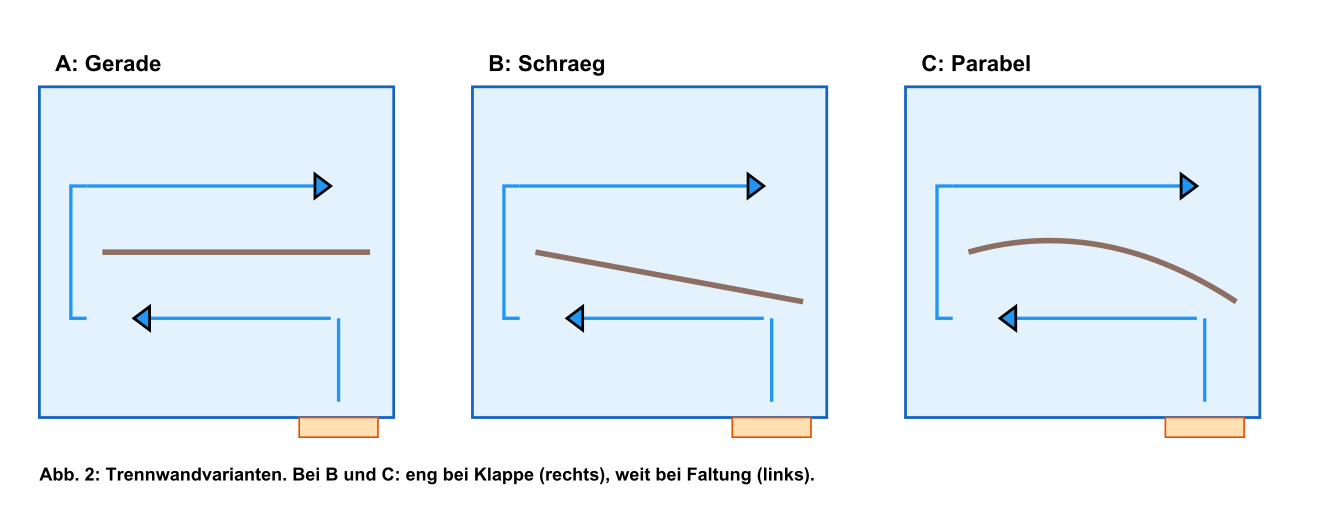
\includegraphics[width=0.85\textwidth]{abb2_varianten.png}
\caption{Dividing wall variants. For B and C: narrow at valve (right), wide at fold (left).}
\end{figure}

All three variants deliver the same volume flow ($\sim$115\,ml/s) and same gap velocity ($\sim$28.8\,m/s) at 1000\,Pa. Reynolds numbers: $\text{Re}_\text{gap} \approx 950$ (laminar), $\text{Re}_\text{channel} \approx 239$ (laminar, $f = 64/\text{Re} = 0.27$). Differences in $\zeta_\text{total}$ are in the per-mille range.

\begin{warnbox}
\textbf{Caution: These results show only the stationary state.} The nearly identical volume flows conceal that the dividing wall decisively affects transient response in practice.
\end{warnbox}

\subsection{Why the Dividing Wall Is Decisive Anyway}

The contradiction resolves when two mechanisms are distinguished -- one dominant and one subordinate:

\textbf{Dominant mechanism: acoustic impedance.} The dividing wall changes the effective acoustic geometry of the chamber: volume distribution between channels, position of the ``acoustic end'' relative to the gap, Helmholtz frequency $f_H$ and quality factor $Q_H$. These changes act via chamber impedance $Z(f)$ on \textbf{both} reeds equally (Chapter 7). The 0°/90°\,test with a simple tube -- without dividing wall, without fold -- shows that solely the position of the chamber opening relative to the gap changes response. The different wall forms (A, B, C) generate different acoustic geometries and thus different $Z(f)$ profiles.

\textbf{Subordinate mechanism: flow guidance (pressure reed only).} In the first milliseconds after valve opening, a pressure pulse runs from the valve through Channel B, around the fold, through Channel A to the gap. The wall form influences how quickly and with what amplitude this pulse arrives at the gap. But this effect acts only on the pressure reed (for the suction reed there is no channel jet) and is subordinate to acoustic coupling, as the practically identical pressure/suction response shows.

\textbf{Stationary flow:} Identical for all three variants. Therefore flow calculation is useful (it confirms the variants do \textit{not} differ stationary), but it does not explain the audible differences.

The three variants thus differ primarily in their \textbf{acoustic effect}:

\textbf{Straight wall (A):} Symmetric channel distribution. Stagnation point generates vortices $\to$ increased dissipation $\to$ lower $Q_H$ $\to$ broader, weaker coupling. Acoustically: uniform impedance profile.

\textbf{Inclined wall (B):} Asymmetric channel distribution (narrow at valve, wide at fold). Less dissipation than A. Changes where acoustic wave encounters different cross-sections $\to$ changes $Z(f)$.

\textbf{Parabolic wall (C):} Continuous cross-section change. Minimal reflections within chamber $\to$ highest $Q_H$ $\to$ narrower, stronger coupling. Acoustically: smoothest impedance transition.

In the electrical engineering analogy: stationary calculation corresponds to the DC resistance of a cable -- nearly equal for all three variants. But \textbf{impedance} at operating frequency (and its overtones) depends on wave impedance, reflections, and dispersion -- which are completely different. For response, DC resistance does not count; the frequency-dependent impedance $Z(f)$ does.

% ============================================================
\section[Dynamic Gap Area]{Dynamic Gap Area -- Why 6\,mm$^2$ Is Only Half the Story}
% ============================================================

All previous calculations use the rest-position gap area $S_\text{gap} = 4\,\text{mm}^2$. But the reed oscillates -- and at full volume the reed tip swings approx.\ 20\,mm downward through the slot. In doing so the reed releases the \textbf{entire slot cross-section}.

\subsection{Geometry of the Through-swing Process}

The slot has width $W_\text{slot} = 9$\,mm and runs through the entire wedge-shaped plate (2--13\,mm thick). The maximum slot cross-section (if the reed were completely removed) is $W_\text{slot} \times t_\text{mean} = 9 \times 7.5 = \mathbf{67.5\,\text{mm}^2}$ -- eleven times the rest-position gap area.

Three phases during through-swing:

\begin{table}[H]
\centering\small
\resizebox{\linewidth}{!}{\begin{tabular}{r l r r r}
\toprule
\textbf{Tip pos.} & \textbf{State} & $S_\text{eff}$ [mm$^2$] & $S/S_\text{rest}$ & \textbf{Released length} \\
\midrule
$+1.5$\,mm & Above plate & 4.5 & 1.1$\times$ & 0\,mm \\
$+0.5$\,mm & Above plate & 1.5 & 0.4$\times$ & 0\,mm \\
$0$\,mm & Gap closes & 7.5 & 1.9$\times$ & 0\,mm \\
$-2$\,mm & In slot & 7.5 & 1.9$\times$ & 0\,mm \\
$-5$\,mm & In slot & 7.5 & 1.9$\times$ & 0\,mm \\
$-10$\,mm & In slot & 7.5 & 1.9$\times$ & 0\,mm \\
$-15$\,mm & Mostly free & 24.7 & 6.2$\times$ & 13\,mm \\
$-20$\,mm & Mostly free & 42.4 & 10.6$\times$ & 28\,mm \\
$-25$\,mm & Mostly free & 49.7 & 12.4$\times$ & 36\,mm \\
$-30$\,mm & Mostly free & 53.7 & 13.4$\times$ & 41\,mm \\
\bottomrule
\end{tabular}}
\caption{Effective flow cross-section at various tip positions}
\end{table}

\textbf{Phase 1 -- Reed above plate ($+1.5$ to $0$\,mm):} Normal gap operation. $S$ decreases from 4.5 to 0\,mm$^2$. Previous calculations apply in this phase.

\textbf{Phase 2 -- Reed in slot ($0$ to $\sim$$-13$\,mm):} Reed plunges into slot. Main cross-section is blocked; only narrow side gaps (0.5\,mm each) remain open. $S$ is limited to approx.\ 7.5\,mm$^2$ (side gap cross-section). This phase is the \textbf{bottleneck in the oscillation cycle}.

\textbf{Phase 3 -- Reed below plate (below $-13$\,mm):} Reed tip has left the slot. From the tip, the full slot cross-section is released ($W_\text{slot} \times t_\text{plate}$). At $-20$\,mm tip: $S_\text{eff} = 42$\,mm$^2$ (\textbf{7-fold}), 28\,mm of reed length are free. At $-30$\,mm: $S_\text{eff} = 54$\,mm$^2$ (\textbf{9-fold}).

\subsection{Time Profile Over the Oscillation Cycle}

\begin{table}[H]
\centering\small
\resizebox{\linewidth}{!}{\begin{tabular}{r r r r r r}
\toprule
\textbf{Ampl.} & $\text{tip}_\text{min}$ & $S_\text{min}$ & $S_\text{max}$ & $S_\text{mean}$ & Mean/$S_\text{rest}$ \\
\midrule
1\,mm & $-0.5$\,mm & 0.0 & 7.5 & 4.3 & 1.1$\times$ \\
2\,mm & $-2.5$\,mm & 0.1 & 7.5 & 5.6 & 1.4$\times$ \\
5\,mm & $-8.5$\,mm & 0.1 & 7.5 & 6.4 & 1.6$\times$ \\
10\,mm & $-18.5$\,mm & 0.1 & 38.8 & 14.9 & 3.7$\times$ \\
15\,mm & $-28.5$\,mm & 0.2 & 52.7 & 25.4 & 6.3$\times$ \\
20\,mm & $-38.5$\,mm & 0.3 & 57.5 & 31.5 & 7.9$\times$ \\
25\,mm & $-48.5$\,mm & 0.0 & 59.9 & 35.4 & 8.8$\times$ \\
\bottomrule
\end{tabular}}
\caption{Time-averaged gap area over one oscillation cycle (all $S$ in mm$^2$)}
\end{table}

\begin{warnbox}
At full volume ($A \sim 20$\,mm), the flow cross-section oscillates between nearly zero and 58\,mm$^2$ -- a \textbf{factor of over 100} within a single oscillation period of 20\,ms. The time-averaged cross-section is 32\,mm$^2$ -- almost \textbf{8 times} the rest-position value (4\,mm$^2$).
\end{warnbox}

\subsection{Consequences for Flow Analysis}

\textbf{1.\ Gap dominates only during start-up:} At the beginning of oscillation (small amplitude) the gap at 4\,mm$^2$ is genuinely the bottleneck -- the chamber with $\sim$950\,mm$^2$ channel cross-section is irrelevant. But once full amplitude is reached, the gap is wide open for a fraction of each half-period. In this phase the chamber, the valve (244\,mm$^2$), and the dividing wall become the relatively narrowest points.

\textbf{2.\ Volume flow pulsates massively:} During a cycle, flow alternates between virtually zero (reed closes gap) and a maximum far exceeding the stationary value (because $S$ is so much larger). Non-stationary volume flow is not a gentle sine signal -- it has extremely steep flanks. These pulses must pass through the chamber.

\textbf{3.\ Chamber becomes a buffer:} The chamber with its volume of approx.\ 180\,cm$^3$ must buffer the extreme volume-flow fluctuations. When the gap briefly allows $10\times$ as much air as in the stationary case, this air must come from somewhere -- from the chamber volume. Chamber pressure drops briefly during each through-swing pulse and is replenished through the valve.

\begin{keybox}
\textbf{4.\ Valve area becomes relevant at full volume:} In the stationary picture the valve with $S_\text{valve}/S_\text{gap} = 61\times$ is completely oversized. But when the gap briefly has 58\,mm$^2$, the ratio is only $S_\text{valve}/S_\text{gap,dyn} = 4.2\times$. This makes valve opening relevant -- and directly explains why a smaller valve opening limits amplitude at full volume (Chapter 5).
\end{keybox}

\textbf{5.\ Dividing wall sees pulsating back-pressure:} During each through-swing phase an underpressure pulse arises in the chamber (air is evacuated through the open gap). This pulse runs back through the chamber to the valve. How the chamber transports this pulse (reflections, damping, dispersion) depends on dividing wall form -- exactly like the pressure pulse during start-up. The dividing wall form thus affects not only start-up but also \textbf{steady-state operation at full volume}.

\begin{keybox}
Stationary calculation with $S_\text{gap} = 4$\,mm$^2$ reliably describes start-up (small amplitude) and gives the correct relations between variants. At full volume the picture changes fundamentally: gap no longer dominates alone, chamber and valve become players, and volume flow becomes extremely pulsating. In this phase chamber geometry becomes relevant even for \textbf{stationary} (time-averaged) resistance -- not only for the impulse response.
\end{keybox}

% ============================================================
\section{Bernoulli Self-Excitation and Start-up Time}
% ============================================================

Self-excitation occurs via the Bernoulli mechanism: if the gap narrows, $v$ rises, $p$ falls, underpressure amplifies deflection. At the reversal point the flow breaks down, the spring drives the reed back.

\begin{figure}[H]
\centering
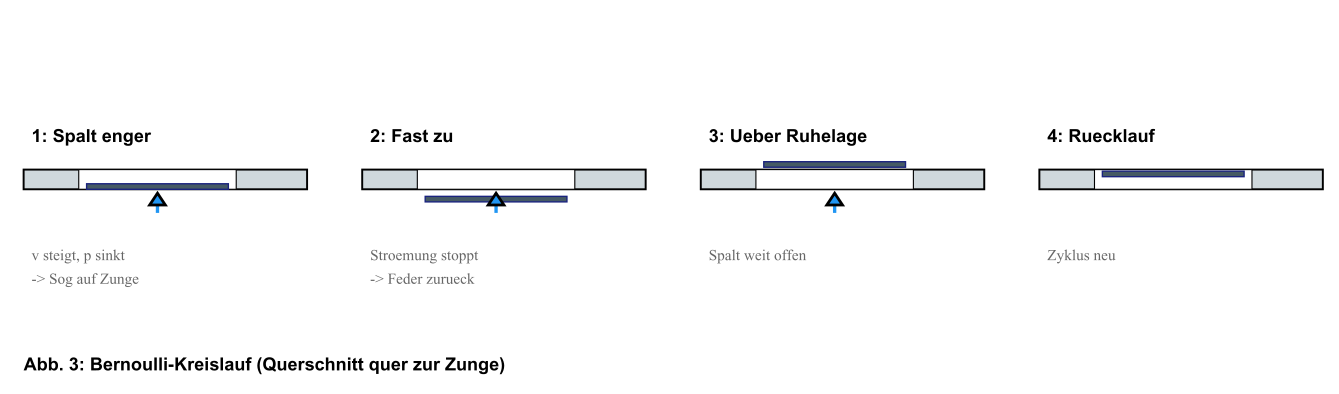
\includegraphics[width=0.85\textwidth]{abb3_bernoulli.png}
\caption{Bernoulli cycle (cross-section transverse to reed).}
\end{figure}

Threshold pressure (v7, correct distributed load on cantilever):
\begin{equation}
\Delta P_\text{min} = \frac{8 E I \cdot h_\text{offset}}{W \cdot L^4} \approx 224\,\text{Pa}
\end{equation}
Low compared to 500--5000\,Pa bellows pressure (v6 had 168\,Pa with incorrect lever arm).

Start-up time $\tau = Q/(\pi f)$ is the actual bottleneck:

\begin{table}[H]
\centering\small
\resizebox{\linewidth}{!}{\begin{tabular}{r r r r}
\toprule
$\zeta$ & $Q$ (quality factor) & $\tau$ [ms] & Periods \\
\midrule
0.005 & 100 & 637 & 100 $\times$ 20\,ms \\
0.01  &  50 & 318 &  50 $\times$ 20\,ms \\
0.02  &  25 & 159 &  25 $\times$ 20\,ms \\
0.04  &  12 &  80 &  12 $\times$ 20\,ms \\
\bottomrule
\end{tabular}}
\caption{Start-up time at 50\,Hz for various quality factors}
\end{table}

$Q$ depends on material, geometry, and clamping and must be measured.

% ============================================================
\section{Static Gap Narrowing Under Bellows Pressure (v8 new)}
% ============================================================

Previous calculation uses the rest-position offset $h_\text{max} = 1.5$\,mm as a fixed value. But \textbf{before} the reed begins to oscillate, bellows pressure is already present. This pressure acts as a distributed load on the cantilever and bends the reed tip downward -- the gap narrows:
\begin{equation}
w_\text{tip}(\Delta p) = \frac{\Delta p \cdot W \cdot L^4}{8EI}, \qquad h_\text{eff} = h_\text{max} - w_\text{tip}(\Delta p)
\end{equation}

\begin{table}[H]
\centering\small
\resizebox{\linewidth}{!}{\begin{tabular}{rrrrrr}
\toprule
$\Delta p$ [Pa] & $\Delta p$ [mbar] & $w_\text{tip}$ [mm] & $h_\text{eff}$ [mm] & $S_\text{gap}$ [mm²] & $S/S_\text{rest}$ \\
\midrule
100 & 1.0 & 0.670 & 0.830 & 2.21 & 0.55 \\
200 & 2.0 & 1.340 & 0.160 & 0.43 & 0.11 \\
224 & 2.2 & 1.500 & 0.020 & 0.05 & 0.01 \\
500 & 5.0 & 3.351 & 0.020 & 0.05 & 0.01 \\
1000 & 10.0 & 6.702 & 0.020 & 0.05 & 0.01 \\
\bottomrule
\end{tabular}}
\caption{Static gap narrowing under bellows pressure (K6). Gap closes above $\Delta p > 224$\,Pa.}
\end{table}

\begin{keybox}
\textbf{Critical pressure:} The gap closes at $\Delta p_\text{crit} = 8EIh_\text{max}/(WL^4) \approx 221$\,Pa $\approx 2.2$\,mbar. This is \textbf{identical} to the threshold pressure $\Delta p_\text{min} = 224$\,Pa -- and not by coincidence: both formulae calculate the same physical effect (distributed load that compensates the offset).
\end{keybox}

In practice, oscillation begins well before $\Delta p_\text{min}$, because Bernoulli instability does not onset only at full static closure:

\textbf{1.\ Dynamic Bernoulli effect:} Already at approx.\ 30--50\,\% of $\Delta p_\text{min}$, flow through the narrowing gap generates enough Bernoulli suction to trigger the first oscillation deflection.

\textbf{2.\ Nonlinear amplification:} Less gap $\to$ higher velocity $\to$ stronger Bernoulli suction $\to$ further narrowing. This positive feedback loop makes the system unstable before static closure.

\textbf{3.\ Estimated onset:} Experience values (Fletcher, Cottingham) show that free-beating reeds typically begin oscillating at 30--50\,\% of static threshold pressure. For this reed: $\Delta p_\text{dyn} \approx 90$\,Pa ($\approx 1$\,mbar). At this pressure the gap is still 60\,\% of rest-position open.

\begin{warnbox}
\textbf{Practical consequence:} Static gap narrowing explains why the effective bellows-pressure range of a reed is limited. Below $\sim 90$\,Pa the reed does not respond; above $\sim 224$\,Pa the gap closes completely. The operating range can be shifted by changing offset: more offset $\to$ higher $\Delta p_\text{crit}$ $\to$ wider range, but also more air consumption at idle.
\end{warnbox}

% ============================================================
\section{Damping -- What It Affects and How}
% ============================================================

Quality factor $Q$ determines start-up time and thus response. $Q$ is not a material constant but the sum of all energy losses per oscillation cycle. These can be decomposed into four physically distinct mechanisms:

\textbf{1.\ Material damping (internal friction):} Every metal converts a fraction of elastic energy to heat when deformed. Loss factor $\eta$ is a material property. For spring steel $\eta$ is 0.0002--0.001, for brass 0.001--0.003. In quality factor decomposition: $Q_\text{material} = 1/\eta$. Spring steel alone achieves $Q_\text{material} \sim 1000$--$5000$, brass 300--1000. Frequency-independent.

\textbf{2.\ Air damping (viscous losses in gap):} The oscillating reed displaces air through the narrow gap (squeeze-film effect). Dissipated power scales with $P_\text{visc} \sim \mu W L^3 \omega^2 a^2 / h^3$. With 1.5\,mm offset the squeeze-film contribution decreases with $h^{-3}$, by factor $(1.5/0.4)^3 \approx 53$ compared to a 0.4-mm gap. Subordinate contribution.

\textbf{3.\ Clamping damping:} At the screw fastening (two screws for bass reeds), energy is microscopically converted to friction during each oscillation. One of the largest individual items. Clean contact surface and uniform screw pressure minimise it.

\textbf{4.\ Sound radiation:} The oscillating reed radiates sound. At 50\,Hz and $70 \times 8$\,mm area the radiation resistance is low (wavelength 6.9\,m). Small contribution for deep bass, increases with $f^2$.

\begin{keybox}
Overall quality factor results from harmonic sum: $\frac{1}{Q_\text{total}} = \frac{1}{Q_\text{mat}} + \frac{1}{Q_\text{air}} + \frac{1}{Q_\text{clamp}} + \frac{1}{Q_\text{rad}}$. For a typical bass reed of spring steel, $Q_\text{total}$ is likely between 50 and 150.
\end{keybox}

$Q$ can be \textbf{lowered} (faster response) by: material choice (brass instead of steel), tip mass loading, smaller offset, softer clamping. $Q$ can be \textbf{raised} (longer sustain, louder tone) by: harder steel, more precise clamping, larger offset. Measurement (decay test) is the only reliable method.

% ============================================================
\section{Lessons from Propeller and Wind Power Aerodynamics}
% ============================================================

\textbf{Trailing edge optimisation:} Wind turbine rotors use serrated trailing edges to reduce tonal noise. At a sharp edge, vortices shed more coherently at a single frequency (Kármán vortices). Serrated edges break up this coherence. The same principle applies to the trailing edge of the dividing wall at the fold gap.

\textbf{Leading edge optimisation:} Humpback whale-inspired leading edges (tubercles) prevent simultaneous flow separation across the entire span. Applied to the chamber: a wavy wall edge (instead of the straight edge of Variant A) could distribute the large-scale separation into many smaller, locally limited separations.

\textbf{Diffuser geometry:} For wind energy diffusers the half-angle must remain below 7°. The inclined dividing wall (Variant B) at 3.7° is safely below this. Continuous curvature (Variant C) is superior to a straight diffuser because the pressure gradient is more evenly distributed.

\begin{keybox}
Transferability has limits: propellers operate at $\text{Re} = 10^5$--$10^7$, the reed chamber at $\text{Re} \sim 50$--$1500$. Nevertheless, geometric principles (continuous curvature, avoiding sharp edges, diffuser angle) are valid independent of Reynolds number.
\end{keybox}

% ============================================================
\section{Why Resonant Chambers Worsen Response}
% ============================================================

A common idea is that a resonant chamber could support the reed -- similar to how a guitar body functions. Practical measurements show the opposite.

The explanation lies in the type of coupling:

\textbf{Parallel coupling} (L and C in parallel): Both elements are excited simultaneously, energy shuttles. Impedance maximum at resonance. A guitar body works this way.

\textbf{Series coupling} (L and C in series): Energy must pass \textit{through} both elements. At resonance total impedance drops, but each element has its own time constant.

\begin{keybox}
The reed chamber is \textbf{series-coupled}. Air must traverse the path bellows $\rightarrow$ valve $\rightarrow$ Channel B $\rightarrow$ fold $\rightarrow$ Channel A $\rightarrow$ slot $\rightarrow$ gap $\rightarrow$ reed in exactly this sequence. Every chamber resonance adds its own time constant to the system.
\end{keybox}

What happens with a resonant chamber? When the Helmholtz frequency is a multiple of the reed frequency, the chamber can co-oscillate. Energy is diverted from the main oscillation into the chamber eigenoscillation. For amplitude build-up this acts like additional damping.

Practical consequence: \textbf{The chamber should be acoustically as \emph{invisible} as possible.} Its eigenfrequencies should lie far from the reed frequency and its overtones. With $f_H = 274$\,Hz (v7: slot as neck, plate thickness as neck length) for a 50-Hz reed, the ratio is 5.5 -- not an integer multiple. This is favourable, but closer to integer multiples than in v6 ($f_H = 461$\,Hz).

Practical experience shows that the dividing wall form decisively affects start-up behaviour -- although all variants deliver nearly identical stationary volume flows. The explanation lies in series coupling: the chamber determines not flow rate but acoustic impedance at the gap.

\begin{keybox}
Optimisation has two levels: the reed itself ($Q$, offset, material) determines fundamental response. Chamber geometry (volume, neck cross-section $\to$ $f_H$) determines the phase of energy supply. Wall form modulates chamber quality factor $Q_H$. Everything must fit together.
\end{keybox}

% ============================================================
\section{Why Phase Determines Response -- Not Flow Quality (v8 new)}
% ============================================================

The previous argument (\emph{clean flow guidance = better response}) is too simplistic. \textbf{What matters is not how evenly the flow arrives at the gap, but whether the energy supply arrives at the reed with the correct phase.} Perfectly even flow helps nothing if phase is wrong.

\textbf{Why no transmission-line model:} The gap-to-channel transition (4\,mm$^2$ $\to$ 950\,mm$^2$) reflects 98.8\,\% of wave energy -- equally for all three variants. A pressure pulse never makes it through this impedance jump as a coherent wave. The chamber does not act as a waveguide but as a \textbf{Helmholtz resonator} with impedance $Z_\text{chamber}(f)$.

Phase of this impedance determines whether energy is pumped into the reed:
\begin{equation}
\text{Phase}(Z) = \arctan\!\left(Q_H \cdot \left(\frac{f}{f_H} - \frac{f_H}{f}\right)\right)
\end{equation}

At $f = f_H$: phase = 0° (resonance, maximum energy exchange). Far below: $\sim -90°$ (compliance). Far above: $\sim +90°$ (mass). For the 50-Hz reed: $f/f_H = 0.18$, phase $\approx -89°$ -- almost pure compliance, the chamber does not disturb the fundamental.

\begin{table}[H]
\centering\small
\resizebox{\linewidth}{!}{\begin{tabular}{rrrrl}
\toprule
Overtone $n$ & $f$ [Hz] & $f/f_H$ & Phase $Z$ [°] & Coupling \\
\midrule
1 &   50 & 0.18 & $-88.5$ & Decoupled \\
5 &  250 & 0.91 & $-52.7$ & Weak \\
6 &  300 & 1.09 & $+51.2$ & Weak \\
8 &  400 & 1.46 & $+79.5$ & Decoupled \\
20 & 1000 & 3.64 & $+87.6$ & Decoupled \\
\bottomrule
\end{tabular}}
\caption{Phase of chamber impedance at overtones of a 50-Hz reed ($f_H = 274$\,Hz, $Q_H \approx 7$)}
\end{table}

No overtone of the 50-Hz reed hits $f_H = 274$\,Hz exactly. The 5th and 6th overtone bracket the resonance with $\sim 53°$ phase offset -- noticeable but not resonant.

\begin{warnbox}
\textbf{What wall form really affects:} Not phase (determined by $f_H$ and $Q_H$) but effective chamber quality factor $Q_H$. Straight wall (A): stagnation point $\to$ energy dissipation $\to$ $Q_H$ drops $\to$ resonance band \textbf{wider} (many overtones weakly affected). Parabolic wall (C): less dissipation $\to$ $Q_H$ higher $\to$ resonance band \textbf{narrower} (few overtones strongly affected). The instrument maker primarily tunes $f_H$ (chamber volume), wall form is fine-tuning of bandwidth.
\end{warnbox}

\subsection{Why the Fold Changes Phase}

The 180°\,fold is an \textbf{acoustic discontinuity}. At the sharp deflection the effective cross-section changes abruptly and flow direction reverses. A pressure pulse is partially reflected there. The reflected portion runs back to the gap and superimposes on the direct chamber pressure.

This superposition is the mechanism: the reflected pulse arrives with a time delay (double fold distance / $c$). Depending on frequency the superposition is constructive or destructive -- the \textbf{effective phase} of chamber pressure at the gap shifts. Additionally, the fold changes the effective acoustic mass of the neck (the air path becomes longer and more convoluted), which slightly shifts $f_H$.

Rounding (quarter-circle) reduces the reflection coefficient at the fold but simultaneously changes the inertance of the bend section (Coltman effect, Section 5.2). A continuous cross-section transition generates less reflection than an abrupt kink -- but also less acoustic shortening. This means: phase comes closer to the ideal Helmholtz value (more predictable) but $f_H$ shifts downward (effective chamber length grows). Whether this improves response depends on where $f_H$ lies relative to reed overtones.

\subsection{Hierarchy of Effects for Response}

Chamber geometry affects response via \textbf{several mechanisms}, physically distinct and of different importance:

\textbf{1.\ Acoustic phase coupling (dominant):} Phase of chamber impedance $Z(f)$ determines whether reed overtones absorb or donate energy to chamber. Determined primarily by $f_H$ (chamber volume, neck cross-section, neck length). Acts on \textbf{both} reeds (pressure and suction) equally. This is the main reason \textbf{chamber size} varies for different pitches.

\textbf{2.\ Acoustic geometry of dividing wall (secondary, but practically relevant):} Dividing wall changes effective acoustic chamber geometry -- where the ``acoustic end'' lies relative to gap, how volume distribution between channels is arranged, and how quality factor $Q_H$ of the resonator turns out. Higher $Q_H$ (less dissipation, e.g.\ Variant C) $\to$ narrower, stronger coupling. Lower $Q_H$ (more dissipation, e.g.\ Variant A) $\to$ broader, weaker coupling. That this effect acts equally on \textbf{both} reeds confirms the acoustic mechanism (Chapter 7). The 0°/90°\,test with unfolded chamber shows that solely position of the chamber end relative to gap changes response -- without dividing wall, without fold.

\textbf{3.\ Flow guidance (subordinate):} Momentum transport through the channel (Chapter 6: tangential component, directional retention) is a real effect, but affects only the pressure reed. Since pressure and suction response are practically indistinguishable and dividing wall form acts equally on both, this mechanism is subordinate to acoustic coupling.

\begin{keybox}
The \textbf{practical experience} of instrument makers that dividing wall form acts audibly is explained primarily by the acoustic mechanism (points 1 and 2): wall form changes $Z(f)$ and $Q_H$, and this change acts on both reeds. Flow effects (point 3) are a real but quantitatively small addition affecting only the pressure reed. For optimisation: chamber geometry (volume, neck) is more important than dividing wall form, and acoustic effect of the dividing wall is more important than its flow-technical effect.
\end{keybox}

% ============================================================
\section{Pre-Chamber Between Valve and Main Chamber (v8 new)}
% ============================================================

What happens when an additional chamber ($48 \times 20 \times 70$\,mm, $V_\text{PC} = 67.2$\,cm$^3$) is built between valve and main chamber? Coupling occurs via an opening with the dimensions of the valve opening ($S = 244$\,mm$^2$).

\subsection{Coupled Helmholtz Resonators}

Two chambers with connecting neck form a coupled two-mass system. The eigenfrequencies split:

\begin{table}[H]
\centering\small
\resizebox{\linewidth}{!}{\begin{tabular}{lrr}
\toprule
& Without PC & With PC \\
\midrule
Mode 1 (in-phase)      & 274\,Hz & 231\,Hz \\
Mode 2 (anti-phase)    & --      & 895\,Hz \\
Anti-resonance         & --      & $\sim$753\,Hz \\
\bottomrule
\end{tabular}}
\caption{Eigenfrequencies without and with pre-chamber (PC)}
\end{table}

\textbf{Mode 1:} Both chambers oscillate in-phase. Reduced 16\,\% from original (274\,Hz) -- the additional volume increases effective compliance. \textbf{Mode 2:} Chambers oscillate anti-phase at 895\,Hz -- far above the relevant range.

\subsection{Phase Shift at the Gap}

\begin{table}[H]
\centering\small
\resizebox{\linewidth}{!}{\begin{tabular}{rrrrl}
\toprule
OT $n$ & $f$ [Hz] & Phase w/o PC & Phase w/ PC & Change \\
\midrule
1 &  50 & $-88.5°$ & $-87.7°$ & $\sim$same \\
5 & 250 & $-52.7°$ & $+41.7°$ & \textbf{better} \\
6 & 300 & $+51.2°$ & $+71.3°$ & worse \\
8 & 400 & $+79.5°$ & $+81.0°$ & $\sim$same \\
\bottomrule
\end{tabular}}
\caption{Phase of chamber impedance at slot, with and without pre-chamber ($Q_H \approx 7$)}
\end{table}

The PC shifts Mode 1 from 274 to 231\,Hz. The 5th overtone (250\,Hz), which without PC lay just below resonance, now sits just above -- phase jumps from $-53°$ to $+42°$ (closer to 0° $\to$ better coupling). The 6th overtone (300\,Hz) moves further from resonance: $+51°$ $\to$ $+71°$ (worse coupling).

\begin{keybox}
\textbf{Practical recommendation:} The pre-chamber is a \textbf{tuning tool}. By varying PC length, Mode 1 can be shifted continuously. Since the PC does not affect stationary flow ($\zeta_\text{coupling}$ relative to gap: $4 \times 10^{-4}$), it is pure acoustic tuning without side effects on fundamental response. Optimum: choose PC length so that an important overtone falls on Mode 1 (phase = 0°).
\end{keybox}

% ============================================================
\section{Which Bass Tones Are Disadvantaged by Chamber Resonance?}
% ============================================================

The Helmholtz frequency of this chamber is 274\,Hz. Which bass tones have an overtone falling near this resonance? As explained in Chapter 10, a resonant chamber extracts energy from the reed via series coupling.

Bandwidth of the Helmholtz resonance depends on its own quality factor $Q_H$. A wooden chamber with valve typically has $Q_H \sim 5$--$10$. At $Q_H = 10$ the critical band is $274 \pm 23$\,Hz, at $Q_H = 5$ it widens to $\pm 27$\,Hz.

\begin{figure}[H]
\centering
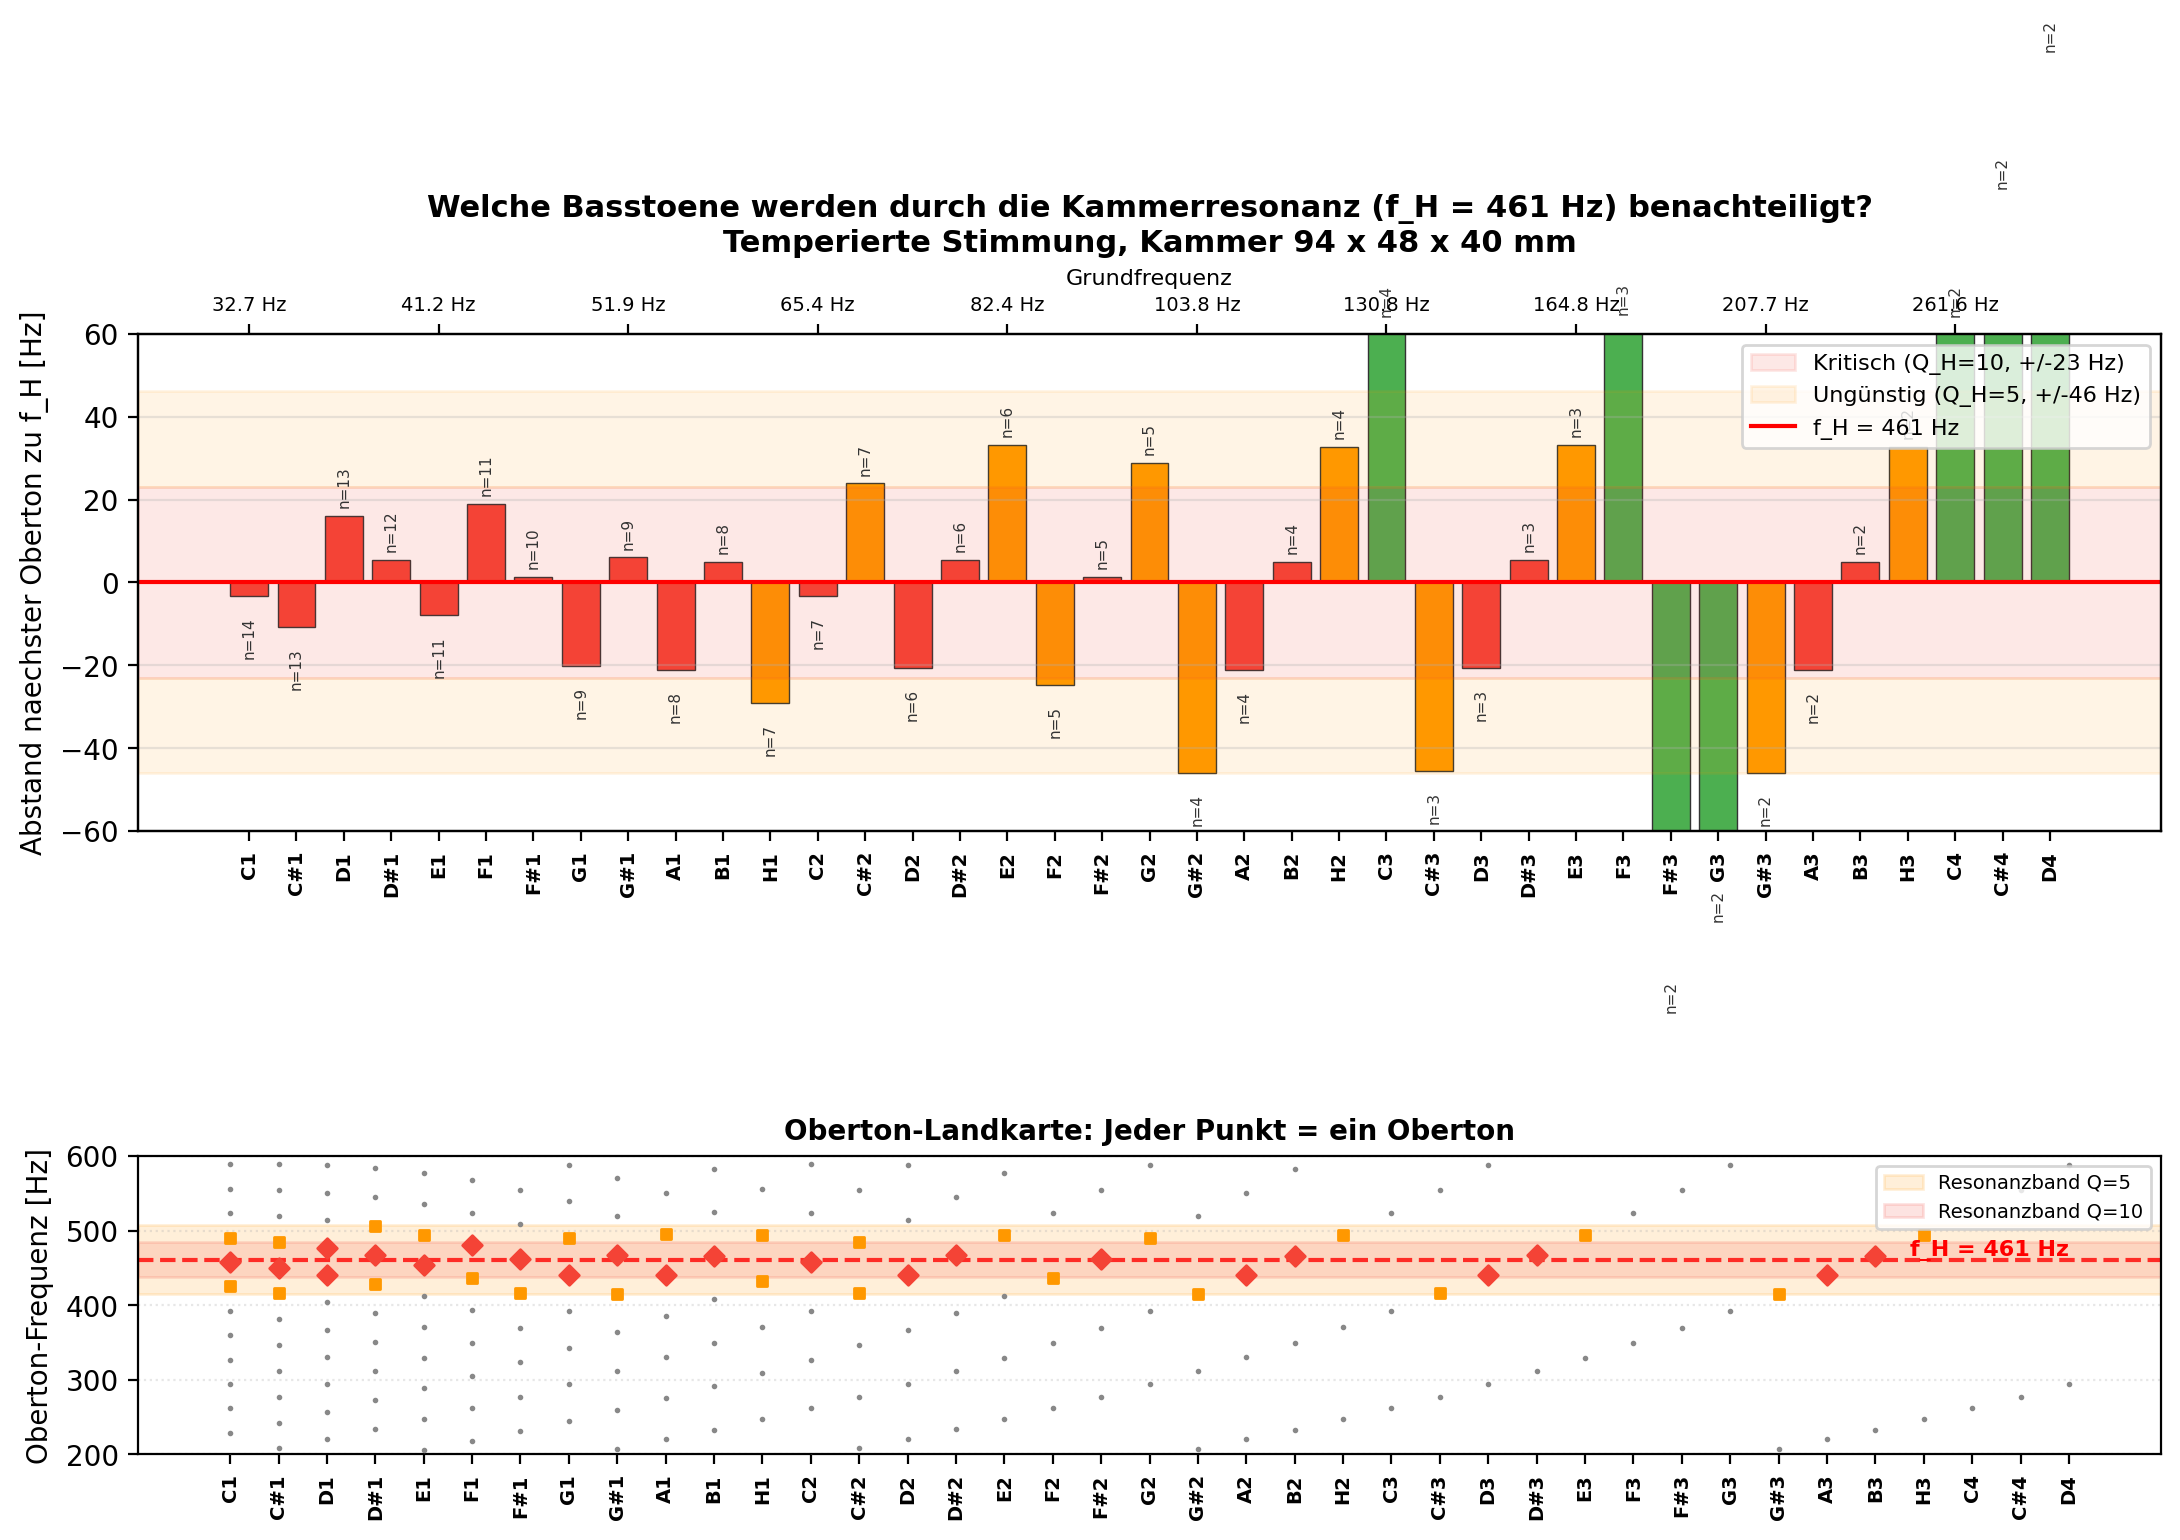
\includegraphics[width=0.9\textwidth]{resonanz_diag.png}
\caption{Upper diagram: distance of nearest overtone to $f_H$. Red = critical, orange = unfavourable, green = unaffected. Lower diagram: overtone map -- each point is an overtone, red diamonds fall within the resonance band.}
\end{figure}

\begin{keybox}
\textbf{Below $\sim$70\,Hz (C2) almost every tone is critically affected.} The reason: at low pitches, overtones lie close together (spacing = fundamental frequency). A 40\,Hz tone has overtones at 40, 80, 120, \ldots, 440, 460, 480\,Hz -- the grid is so fine that an overtone always falls within the resonance band. The lower the pitch, the more unavoidable the conflict.
\end{keybox}

Particularly affected are tones whose fundamental frequency is an integer divisor of $f_H$:

\begin{table}[H]
\centering\small
\resizebox{\linewidth}{!}{\begin{tabular}{l r l r r}
\toprule
$f_H / n$ & $f$ [Hz] & Nearest note & Difference & Overtone $n$ \\
\midrule
274/2 & 137.0 & C3 (130.8) & $+6.2$\,Hz & 2 \\
274/3 &  91.3 & F2 (87.3)  & $+4.0$\,Hz & 3 \\
274/4 &  68.5 & C2 (65.4)  & $+3.1$\,Hz & 4 \\
274/5 &  54.8 & A1 (55.0)  & $-0.2$\,Hz & 5 \\
274/6 &  45.7 & F1 (43.6)  & $+2.0$\,Hz & 6 \\
274/7 &  39.1 & E1 (41.2)  & $-2.1$\,Hz & 7 \\
274/8 &  34.2 & C1 (32.7)  & $+1.5$\,Hz & 8 \\
274/9 &  30.4 & C1 (32.7)  & $-2.3$\,Hz & 9 \\
\bottomrule
\end{tabular}}
\caption{Integer divisors of $f_H$ and corresponding bass tones}
\end{table}

Above C3 (130.8\,Hz) no divisor lies close enough. But below -- especially A1 (divisor 5, deviation only $-0.2$\,Hz!) and F1 (divisor 6) -- there are critical tones. At $Q_H = 5$ the resonance band is $274 \pm 27$\,Hz wide, i.e.\ 247--301\,Hz. The lowest bass tones have overtones so closely spaced that an overtone almost always falls within the band.

% ============================================================
\section{What Calculations Can and Cannot Achieve}
% ============================================================

The presented calculations are based on well-established physical models: Euler-Bernoulli beam theory for reed frequency, Bernoulli equation for gap flow, Helmholtz resonator for chamber acoustics, loss coefficients from fluid mechanics (Idelchik). These models give results of the right order of magnitude.

Nevertheless they do not replace practical testing:

\textbf{1.\ Idealised geometry:} Exactly plane surfaces, sharp edges, uniform gaps. In reality: wood grain, machining marks, individual offsets. Even 0.1\,mm difference in offset changes $S_\text{eff}$ by $\sim$7\,\%.

\textbf{2.\ Stationary flow:} \textbf{This is the most serious limitation.} Loss calculation assumes stationary flow. In reality the flow pulsates at 50\,Hz. Practical experience shows that dividing wall form decisively affects start-up behaviour. The dominant mechanism is \textbf{acoustic} (impedance coupling $Z(f)$, acts on both reeds equally, see Chapter 7), not fluid-mechanical. Stationary calculation captures neither acoustic nor transient effects.

\textbf{3.\ Damping:} $Q$ is the most sensitive parameter. Differences of factor 2 between apparently identical reeds are normal.

\textbf{4.\ Chamber acoustics:} The Helmholtz model is simplified. In reality the chamber has further modes, and acoustic properties change with bellows pressure, temperature, and humidity.

\textbf{5.\ Interactions:} Every effect is modelled individually. A complete solution would require coupled fluid-structure-acoustics simulation (FSI).

Calculations reliably identify which parameters matter and at which level they act. They rank the three dividing wall variants in a physically justified order (C better than B better than A -- confirmed by practical experience). Where calculation reaches its limits is the quantitative prediction of the wall effect: that the wall acts is physically justifiable. How strongly -- can only be measured.

\begin{keybox}
For the instrument maker this means: \textbf{Calculation says where to look. Practical testing says what to find.} Together, both are more than either alone.
\end{keybox}

% ============================================================
\section{Summary}
% ============================================================

\begin{itemize}[leftmargin=5mm, itemsep=3pt]
\item \textbf{Reed plate:} Wedge-shaped (2$\rightarrow$13\,mm). At the free end, the 13-mm slot acts as a short channel with its own flow resistance ($\zeta \approx 1.62$, including $\zeta_\text{entry} = 0.5$ entry loss [K3b]).

\item \textbf{Gap:} Triangular (0$\rightarrow$1.5\,mm), $S_\text{eff} = W \cdot h/3 = 4$\,mm$^2$. Dominates total resistance. All variants: $v \approx 29$\,m/s, $Q \approx 115$\,ml/s at 1\,kPa.

\item \textbf{Dynamic gap change [K6]:} Bellows pressure bends reed statically downward. Critical pressure $\Delta p_\text{crit} = 221$\,Pa $\equiv$ threshold pressure. Effective oscillation onset at $\sim 90$\,Pa (1\,mbar). Operating range 90--224\,Pa.

\item \textbf{Wall material:} Film and veneer are equivalent from a flow perspective. Veneer is more stable and acoustically more neutral.

\item \textbf{Valve orientation:} Blow-out ($\zeta = 0.66$) better than deflect ($\zeta = 1.86$). Blow-out fully utilises wall geometry.

\item \textbf{Dividing wall form:} Practically decisive for response (non-stationary start-up). C (parabola) best directional retention, B (inclined) good compromise, A (straight) simplest but most sluggish. Stationary flow equal for all -- the difference lies in impulse response (reflections, directional loss). Turbulence for self-excitation is generated by the gap itself.

\item \textbf{Response:} $\tau = Q/(\pi f)$. At $Q = 100$: 637\,ms, at $Q = 25$: 159\,ms. Chamber geometry does not affect stationary flow but decisively affects non-stationary start-up.

\item \textbf{Acoustics:} Helmholtz 274\,Hz, chamber acoustically small.

\item \textbf{Phase coupling (v8 new):} Response by three mechanisms: (1) acoustic phase (dominant, via $f_H$), (2) acoustic geometry of dividing wall ($Q_H$, volume distribution, position of acoustic end -- acts on both reeds), (3) flow guidance (subordinate, pressure reed only).

\item \textbf{Pre-chamber (v8 new):} $48 \times 20 \times 70$\,mm (67\,cm$^3$) lowers Mode 1 from 274 to 231\,Hz ($-16\,\%$). PC length is tuning tool for overtone phase without effect on stationary flow.
\end{itemize}

\end{document}
